\begin{figure*}[h]
	\begin{subfigure}{0.48\textwidth}
		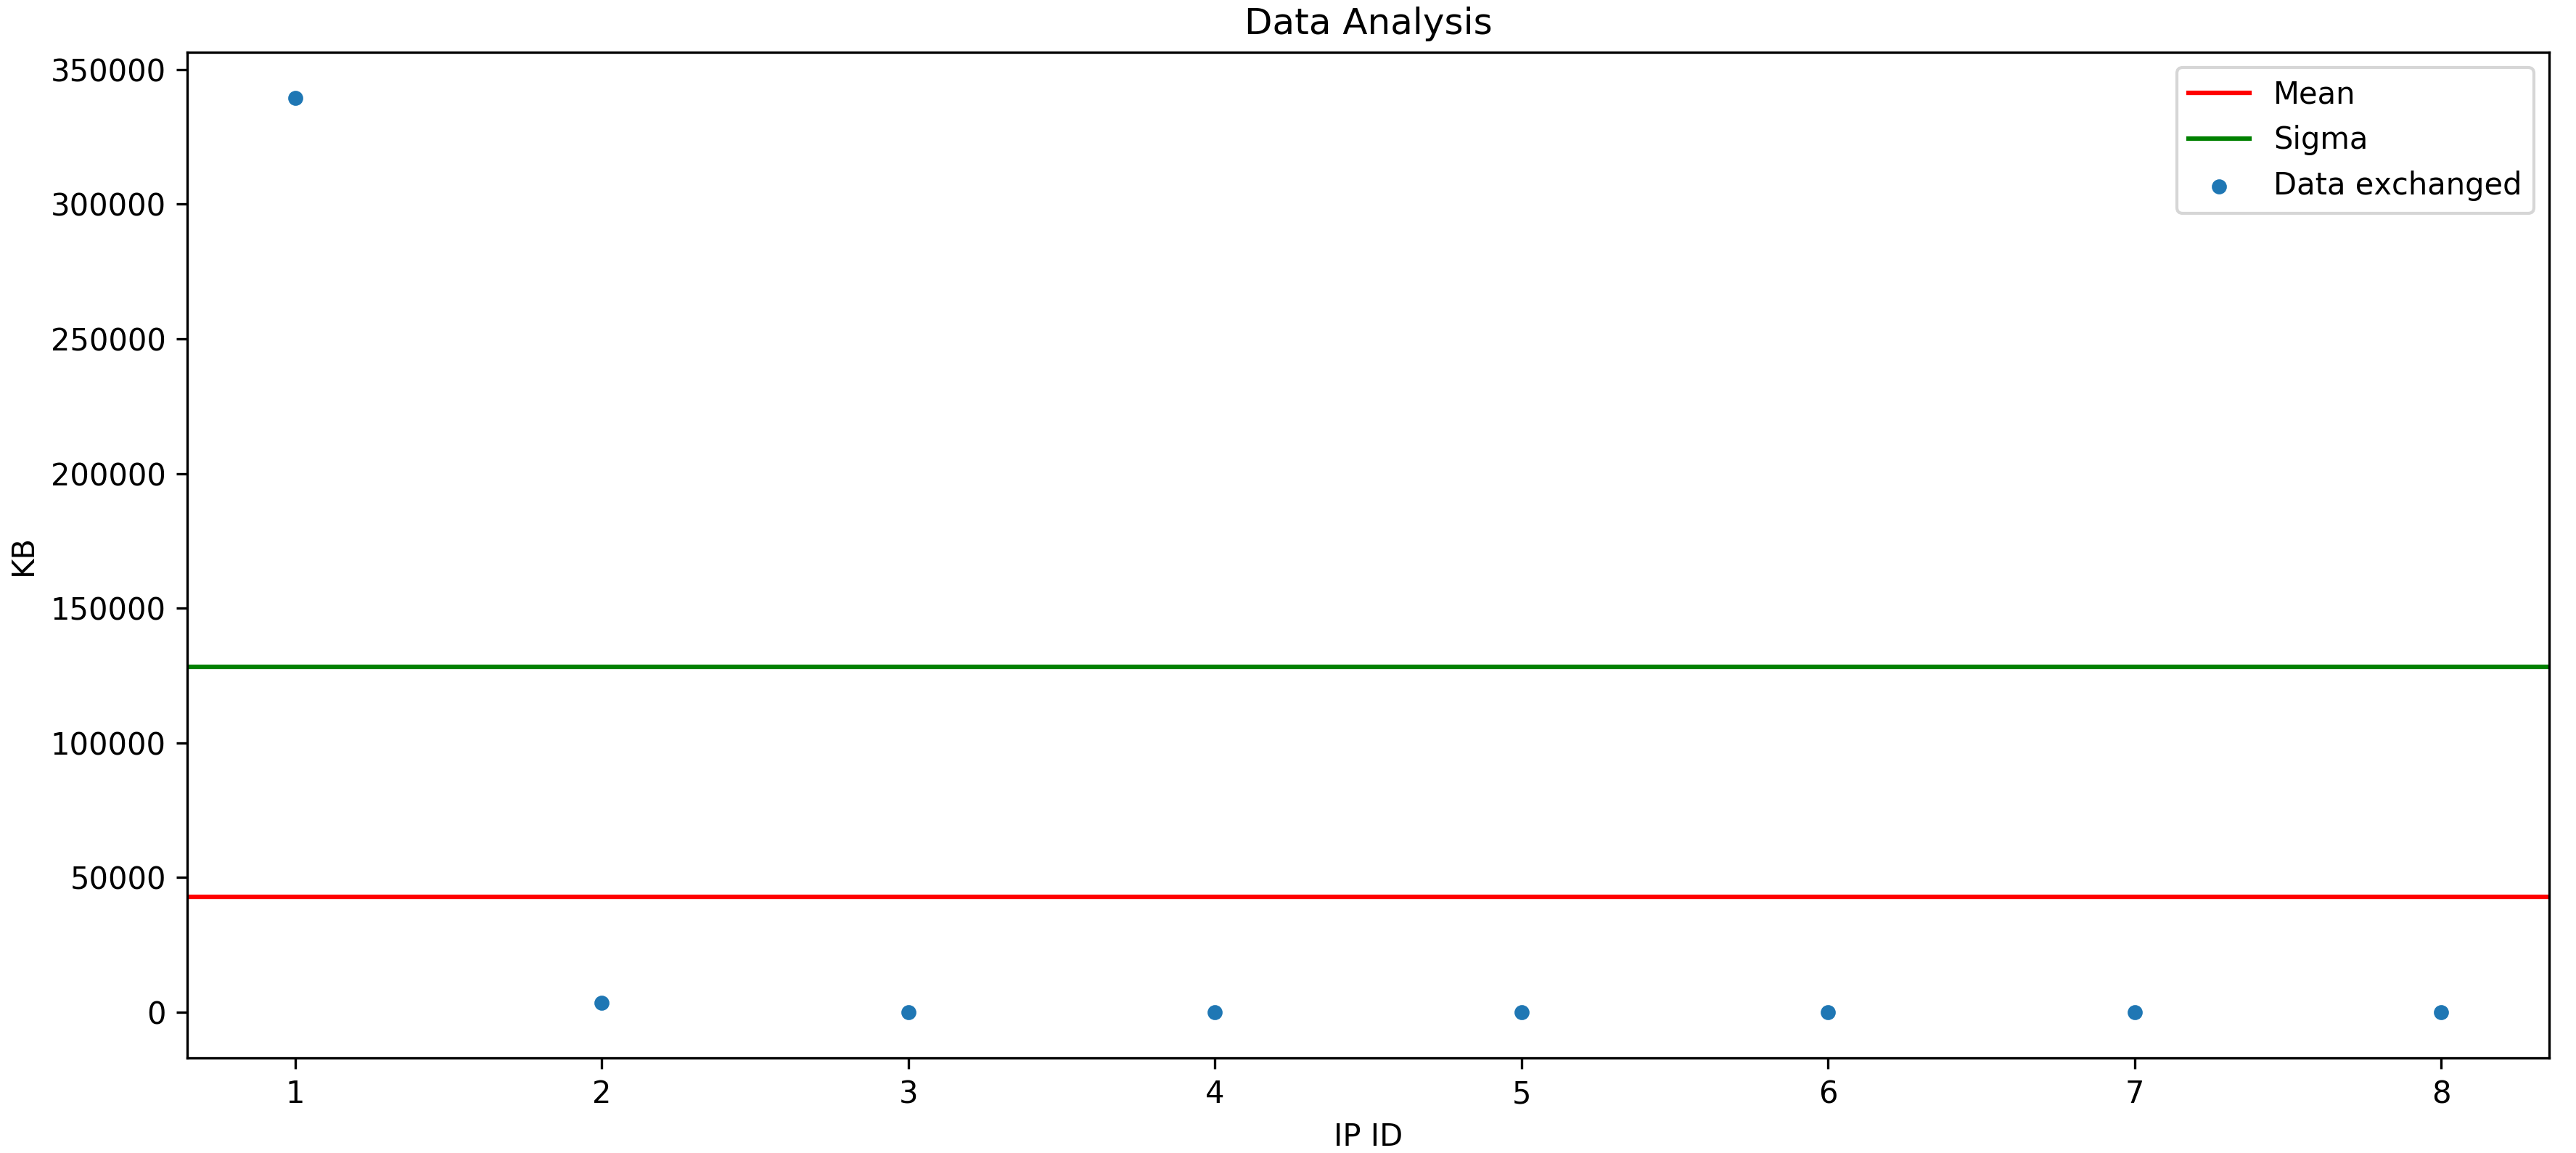
\includegraphics[width=\textwidth]{imgs/DoSMixed-data_analysis.png}
  		\caption{DoS Data Analysis}
  		\label{fig:ddos_data}
	\end{subfigure}
	\hspace*{\fill} % separation between the subfigures
	\begin{subfigure}{0.48\textwidth}
  		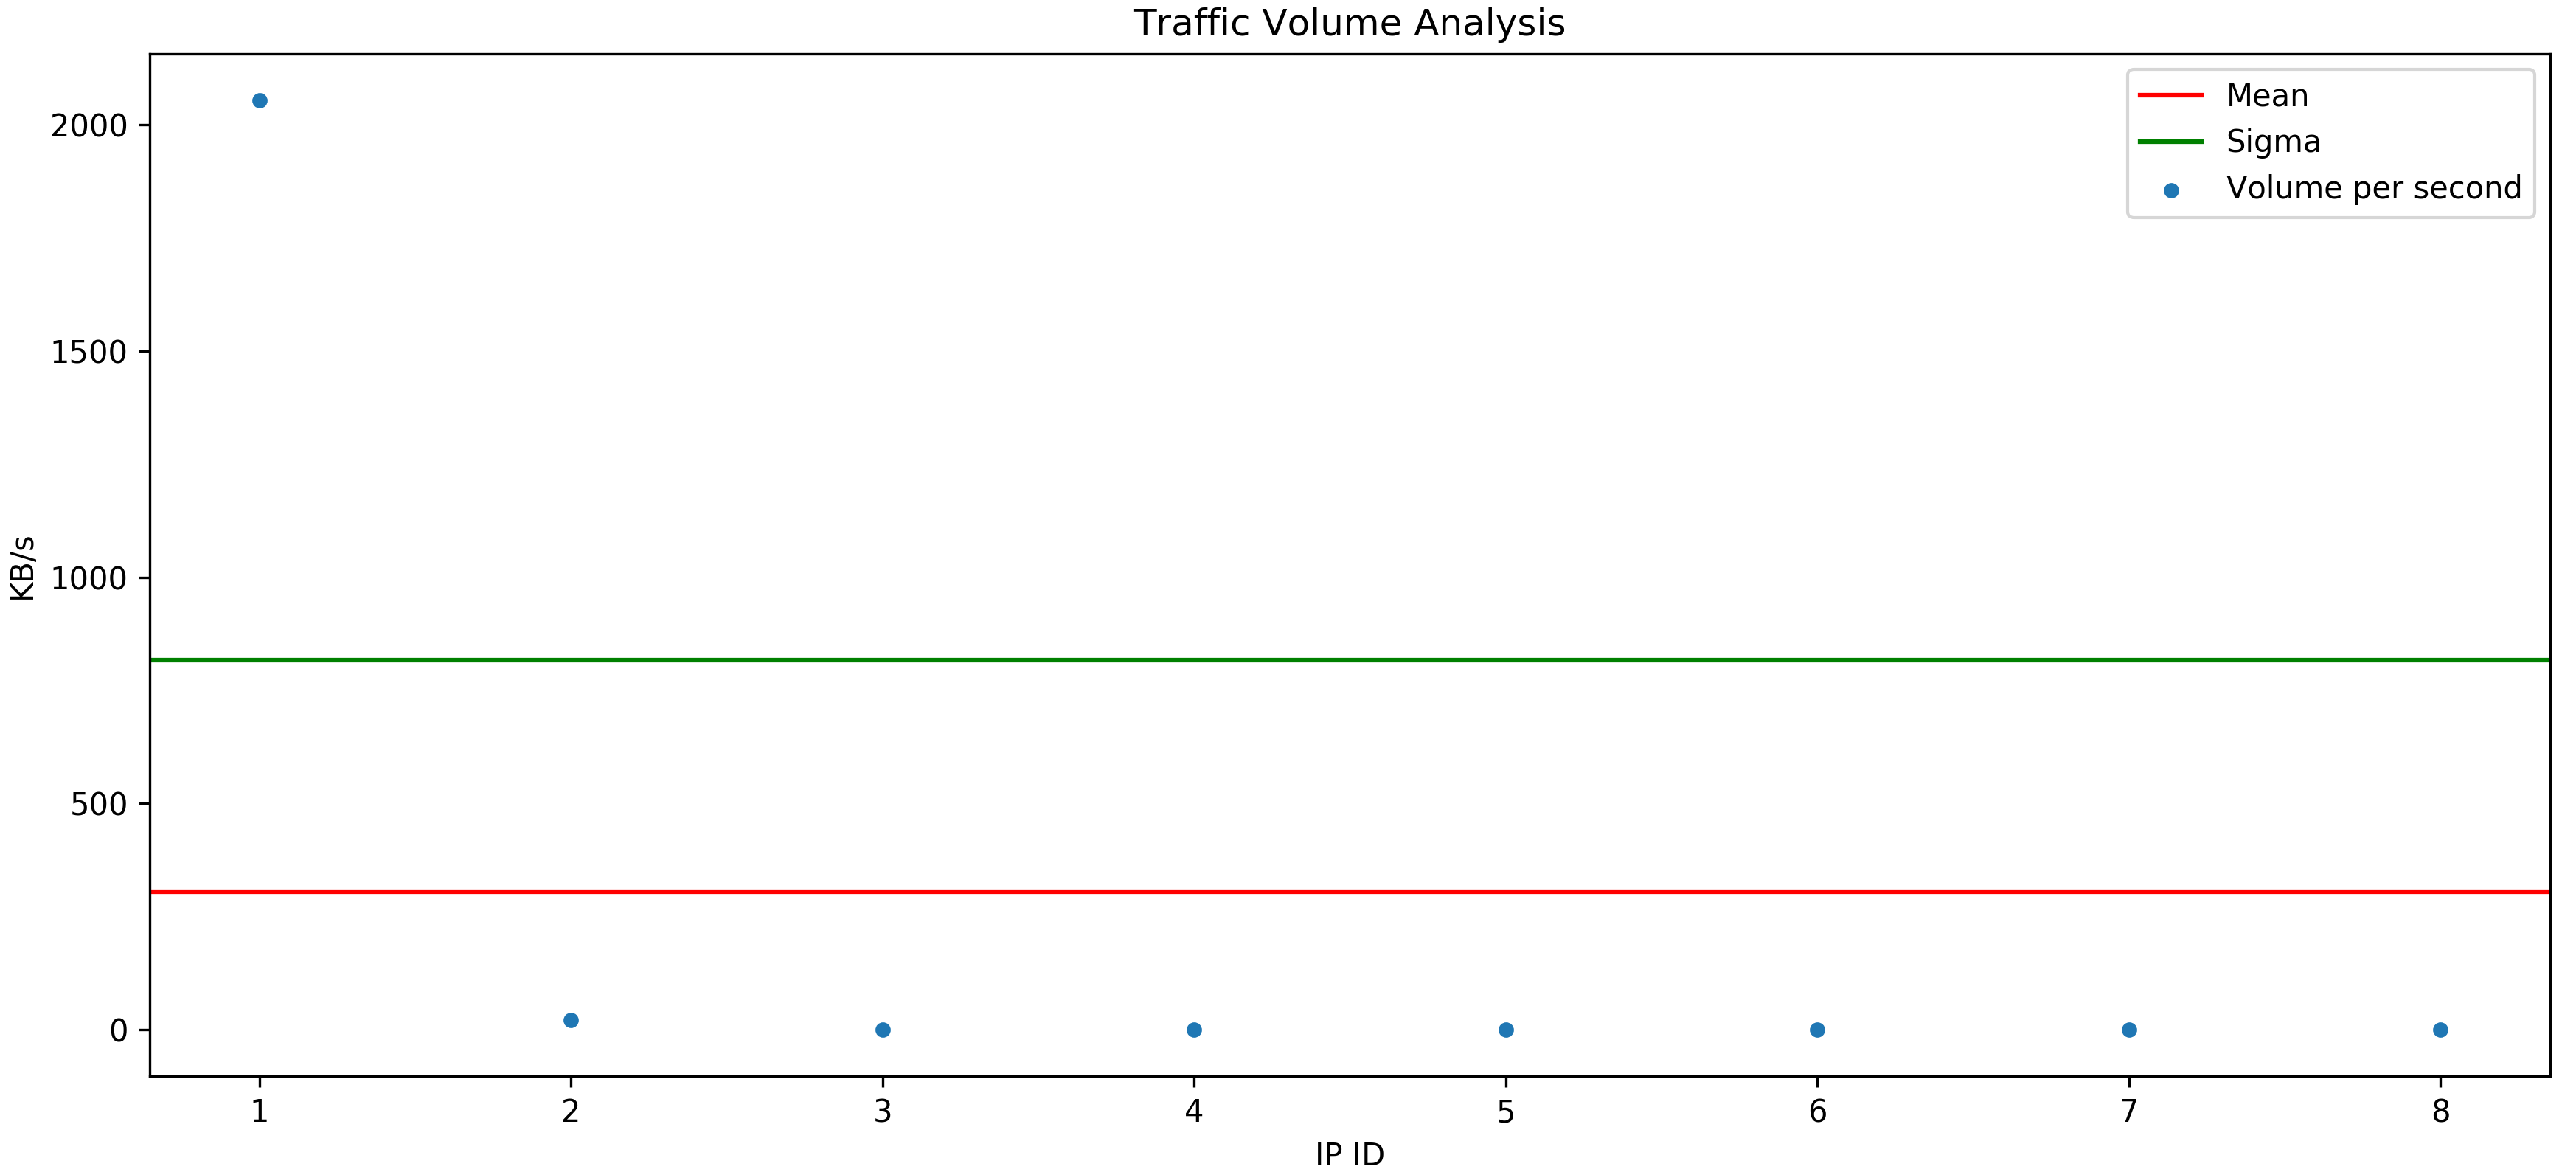
\includegraphics[width=\textwidth]{imgs/DoSMixed-volume_analysis.png}
  		\caption{DoS Volume Analysis}
  		\label{fig:dos_volume}
	\end{subfigure}
	\caption{DoS attack Analysis}
	\label{fig:dos_analysis}
\end{figure*}

\section{Analysis}
\label{sec:analysis}
In this section we will illustrate the testbed on which we have tested our tool, traffic analysis is mainly based on IP addresses and timestamp \cite{ddos_forensics}. 
More over we will show two examples of attack, DDoS and DoS, in order to explain and evaluate our analysis quality.
For the reliability estimation of our tool we used different datasets\footnote{Some datasets were generated by our tool, it is possible to analyse every type of dataset on your own if in \texttt{pcap} format and converted using our tool.} to justify our conclusions. 
Two datasets were generated by our tool and other two were generated over our implemented testbed, these last two will recreate a realistic scenario.
%% TODO VEDERE SE POSSIBILE CORRELAZIONE TRA REGISTRAZIONI LEGIT E SOTTO ATTACCO, VEDERE SE SI PUO USARE CORRELAZIONE PER DIRE CHI STA ATTACCANDO.
There is also a summary of how to configure and run an analysis with \textit{Python} and \textit{Hadoop}.

\subsection{Configuring and Running Analysis}
This tool has been developed for running analysis over network flow records with minimal effort from the user. Once installed and configured \textit{Hadoop} on your PC or cluster, only one line of code is needed for running and storing the results of an analysis\footnote{Is assumed that the dataset is pre-loaded into the Hadoop file system.}, as shown in the example below

\begin{lstlisting}[firstline=1, lastline=1]
   python3 DDoSAnalysis.py -a dataset_name
	Write('Case insensitive '); 
	Write('Bash keywords.')
\end{lstlisting}

\subsection{Testbed} 
The created testbed is illustrated in Fig.\ref{fig:networkscenario}, as we can see it is a very simple and basic design scenario. There is a \textit{router} that communicates with \textit{internet},  it connects the \textit{sever} with the global network, as we will see further on the treatment \textit{internet} may contains one or several attackers which aim is to deny the service given by the \textit{server}. 

The \textbf{Server} in our testbed was created deploying an UDP service on a MacBook Pro, it has an 2,6 GHz Intel Core i5 processor and 8 GB of RAM memory. 
We used \textit{Wireshark}, which is the world's foremost and widely-used network protocol analyser, to record network flow passing through our server. 
Wireshark creates a \textit{log} file that will be analysed by our tool in order to detect possible attacks.

Our UDP service used in this testbed is a very simple, it receives UDP packets which contain text, and it saves received text inside a file.
Users can send text to the server, we implemented a script for legitimate users, it simulate human user time of writing by waiting random time between one to ten seconds before send it to the server.
We also created a script which aim is to attack the server, it implements \textit{UDP flood} attack, its code is very simple, it consists in a \texttt{while} cycle in which we create an UDP packet containing random strings and we send it to the server.
We launched our user\footnote{Plots showed in Fig. \ref{fig:dos_analysis} and Fig. \ref{fig:ddos_analysis} has more IP then the specified ones because of external traffic of the host machine, as we can se they are irrelevant in our analysis} simulating script on four computers in order to get standard traffic values from legittimate users, once got it we started launching DoS and DDoS attacks. During DDoS there were three computer interacted with the server then two attacker flooded the server overwhelming it.    

The aim of this testbed is to recreate a valid and realistic simulation of a real scenario in order to verify the reliability of our analysis tool. 
We do not complicate network structure in order to concentrate our heed on the implementation of analysis tools and big data scripting, which are the main topics of this project.
  
\subsection{DoS Analysis Example}
A DoS attack is a common way to saturate the server bandwidth. It's often used in combination with other vulnerabilities to amplificate the DoS traffic volume, as we have seen in the wild with the Memcached vulnerability\cite{memcached_vulnerability}. 
In our example, Fig. \ref{fig:DoS}, we don't consider the possibility to track the real culprit behind a proxy.

During this simulation we start recording network flow on or server while legitimate users were active, then after more less three thousand, of various type, exchanged packets recorded we start the DoS attack and we register an income flow of 350 Mbps for a few seconds then the server crashes and the income flow decreases but the attacker was still overwhelming the server.
Standard deviation works well for detecting anomalies in data that is normally distributed, we used it to identify which series deviate greatly from their usual behaviour ...
%% TODO descrivere come � stato rilevato attaccante
We can immediately see in Fig. \ref{fig:dos_analysis} how the attacker with \textit{id 0} is immediately recognised because of a huge amount of traffic volume and a large spike in packet speed. 

Here, in the two graphs, we can see the mean value, represented in a red line: the attacker distance from the sigma value is also more accentuated in both graphs, which suggests an involvement in the DoS genesis.

\subsection{DDoS Analysis Example}
DDoS is a popular approach for attackers to paralyse computers or network systems by coordinating flooding traffic originated from multiple hosts simultaneously, to block legitimate users' system access by reducing resource availability. 
DDoS attack inherits similar characteristics of DoS attacks, with the differences in an increased scale which in term yields a higher impact\cite{ddos_forensics}.

In our attack scenario, Fig. \ref{fig:DDoS},  the attacker controls a botnet of two devices.
By using \textit{UDP flood} attack the botmaster unleash his botnet against the server for few seconds overwhelming it. 
During this attack we recorded an income flow of 350-380 Mbps, that is sufficient in order to get down our server, as we have seen in the previous subsection the income flow is more less the same and we empirically suppose that is the upper bound of data which the server\footnote{The server is wireless connected to the network.} can deal with.
Launching our analysis tool, thanks to its big data features, we are capable to deal with the \texttt{ddos\_log} file easily.

The analysis results are shown in Fig. \ref{fig:ddos_analysis}, as we can see there are two  visible clusters, one of legitimate users and one of attackers. 
We can easily recognise attackers from legitimate users because the data exchanged in terms of KB is very high (fig. \ref{fig:ddos_data}) like also the traffic generated in therms of KB over seconds is high (fig. \ref{fig:ddos_volume}) respect the average of norma traffic on the server in normal conditions. 
%% TODO descrivere come sono trovati gli attaccanti usando matematica.

Our tool output also a dataset which contains the IP and all the statistics previously mentioned, in this dataset we can retrive the IP of the attacker by its id which is used to identify it into the output figures. 
